%----------------------------------------------------------------------------------------
%	PACKAGES AND OTHER DOCUMENT CONFIGURATIONS
%----------------------------------------------------------------------------------------

\documentclass[12pt]{article}
%\usepackage[spanish]{babel} %Tildes
\usepackage[extreme]{savetrees} %Espaciado e interlineado. Comentar si no gusta el interlineado.
\usepackage[utf8]{inputenc} %Encoding para tildes
\usepackage[breakable,skins]{tcolorbox} %Cajitas
\usepackage{fancyhdr} % Se necesita para el título arriba
\usepackage{lastpage} % Se necesita para poner el número de página
\usepackage{amsmath,amsfonts,amssymb,amsthm} %simbolos y demás
\usepackage{mathabx} %más símbolos
\usepackage{physics} %simbolos de derivadas, bra-ket.
\usepackage{multicol}
\usepackage[customcolors]{hf-tikz}
\usepackage[shortlabels]{enumitem}
\usepackage{tikz}

%\def\darktheme
%%%%%%%%% === Document Configuration === %%%%%%%%%%%%%%

\pagestyle{fancy}
\setlength{\headheight}{14.49998pt} %NO MODIFICAR
\setlength{\footskip}{14.49998pt} %NO MODIFICAR

\ifx \darktheme\undefined

\lhead{Math161S1} % Nombre de autor
\chead{\textbf{Week 3.1}} % Titulo
\rhead{}%\firstxmark} 
\lfoot{}%\lastxmark}
\cfoot{}
\rfoot{Page \thepage\ of\ \pageref{LastPage}} %A la derecha saldrá pág. 6 de 9. 
\else
\pagenumbering{gobble}
\pagecolor[rgb]{0,0,0}%{0.23,0.258,0.321}
\color[rgb]{1,1,1}
\fi

%%%%%%%%% === My T Color Box === %%%%%%%%%%%%%%

\ifx \darktheme\undefined
\newtcolorbox{ptcb}{
colframe = black,
colback = white,
breakable,
enhanced
}
\newtcolorbox{ptcbP}{
colframe = black,
colback = white,
coltitle = black,
colbacktitle = black!40,
title = Practice,
breakable,
enhanced
}

\else
\newtcolorbox{ptcb}{
colframe = white,
colback = black,
colupper = white,
breakable,
enhanced
}
\newtcolorbox{ptcbP}{
colframe = white,
colback = black,
colupper = white,
coltitle = white,
colbacktitle = black,
title = Practice,
breakable,
enhanced
}
\fi

%%%%%%%%% === Tikz para matrices === %%%%%%%%%%%%%%

\tikzset{
  style green/.style={
    set fill color=green!50!lime!60,
    set border color=white,
  },
  style cyan/.style={
    set fill color=cyan!90!blue!60,
    set border color=white,
  },
  style orange/.style={
    set fill color=orange!80!red!60,
    set border color=white,
  },
  row/.style={
    above left offset={-0.15,0.31},
    below right offset={0.15,-0.125},
    #1
  },
  col/.style={
    above left offset={-0.1,0.3},
    below right offset={0.15,-0.15},
    #1
  }
}

%%%%%%%%% === Theorems and suchlike === %%%%%%%%%%%%%%

\theoremstyle{plain}
\newtheorem{Th}{Theorem}  %%% Theorem 1.1
\newtheorem*{nTh}{Theorem}             %%% No-numbered Theorem
\newtheorem{Prop}[Th]{Proposition}     %%% Proposition 1.2
\newtheorem{Lem}[Th]{Lemma}             %%% Lemma 1.3
\newtheorem*{nLem}{Lemma}               %%% No-numbered Lemma
\newtheorem{Cor}[Th]{Corollary}        %%% Corollary 1.4
\newtheorem*{nCor}{Corollary}          %%% No-numbered Corollary

\theoremstyle{definition}
\newtheorem*{Def}{Definition}       %%% Definition 1.5
\newtheorem*{nonum-Def}{Definition}    %%% No number Definition
\newtheorem*{nEx}{Example}             %%% No number Example
\newtheorem{Ex}[Th]{Example}           %%% Example
\newtheorem{Ej}[Th]{Exercise}         %%% Exercise
\newtheorem*{nEj}{Exercise}           %%% No number Excercise
\newtheorem*{Not}{Notation}       %%% Definition 1.5

\theoremstyle{remark}
\newtheorem*{Rmk}{Remark}      %%%Remark 1.6

%\numberwithin{equation}{section}

\setlength{\parindent}{3ex}

%%====== Useful macros: =======%%%

\DeclareMathOperator{\gen}{gen}     %%%set generated by...
\DeclareMathOperator{\Rng}{Rng}     %%%rangomat
\DeclareMathOperator{\Nul}{Nul}     %%%rangomat
\DeclareMathOperator{\Proy}{Proy}   %%%proyección
\DeclareMathOperator{\id}{id}       %%%identity operator

\newcommand{\al}{\alpha}            %%%short for \alpha
\newcommand{\la}{\lambda}           %%%short for \lambda
\newcommand{\sg}{\sigma}            %%%short for \sigma
\newcommand{\te}{\theta}                %% short for  \theta
\renewcommand{\l}{\ell}

\newcommand{\thickhat}[1]{\mathbf{\hat{\text{$#1$}}}}
\newcommand{\ii}{\vu{\imath}}
\newcommand{\jj}{\vu{\jmath}}
\newcommand{\kk}{\thickhat{k}}

\newcommand{\bC}{\mathbb{C}}        %%%complex numbers
\newcommand{\bN}{\mathbb{N}}        %%%natural numbers
\newcommand{\bP}{\mathbb{P}}        %%%polynomials
\newcommand{\bR}{\mathbb{R}}        %%%real numbers
\newcommand{\bZ}{\mathbb{Z}}        %%%integer numbers
\newcommand{\cB}{\mathcal{B}}       %%%basis
\newcommand{\cC}{\mathcal{C}}       %%%basis
\newcommand{\cM}{\mathcal{M}}       %%%matrix family

\newcommand{\sT}{\mathsf{T}}        %%%traspuesta

\renewcommand{\geq}{\geqslant}      %%%(to save typing)
\renewcommand{\leq}{\leqslant}      %%%(to save typing)
\newcommand{\x}{\times}             %%%product
\renewcommand{\:}{\colon}           %%%colon in  f: A -> B
\newcommand{\isom}{\simeq}              %% isomorfismo

\newcommand{\un}[1]{\underline{#1}}
\newcommand{\half}{\frac12}

\newcommand*{\Cdot}{{\raisebox{-0.25ex}{\scalebox{1.5}{$\cdot$}}}}      %% cdot más grande
\renewcommand{\.}{\Cdot}                %% producto escalar

\newcommand{\twobyone}[2]{\begin{pmatrix} %% 2 x 1 matrix
  #1 \\ #2 \end{pmatrix}}
  \newcommand{\twobytwo}[4]{\begin{pmatrix} %% 2 x 2 matrix
    #1 & #2 \\ #3 & #4 \end{pmatrix}}
    \newcommand{\twobythree}[6]{\begin{pmatrix} %% 2 x 3 matrix
        #1 & #2 & #3\\ #4 & #5 & #6 \end{pmatrix}}
\newcommand{\threebyone}[3]{\begin{pmatrix} %% 3 x 1 matrix
  #1 \\ #2 \\ #3 \end{pmatrix}}
  \newcommand{\threebytwo}[6]{\begin{pmatrix} %% 3 x 1 matrix
    #1 & #2\\ #3 & #4\\ #5&#6 \end{pmatrix}}
\newcommand{\threebythree}[9]{\begin{pmatrix} %% 3 x 3 matrix
  #1 & #2 & #3 \\ #4 & #5 & #6 \\ #7 & #8 & #9 \end{pmatrix}}

\newcommand{\To}{\Rightarrow}

\newcommand{\vaf}{\overrightarrow}

\newcommand{\set}[1]{\{\,#1\,\}}    %% set notation
\newcommand{\Set}[1]{\biggl\{\,#1\,\biggr\}} %% set notation (large)
\newcommand{\red}[1]{\textcolor{red}{#1}}
\newcommand{\blu}[1]{\textcolor{blue}{#1}}

%----------------------------------------------------------------------------------------
%	ARTICLE CONTENTS
%----------------------------------------------------------------------------------------

\begin{document}
\begin{multicols}{2}
\section*{Improper Integration}

The integral of a function $f$ represents the area enclosed by $f$'s graph and the $x$ axis.\par 
We have studied this type of integrals and these are called \emph{definite integrals}. But what happens when there's a discontinuity in the function? Or when we want to find an infinite area? These questions are illustrated in the following examples:
$$\int_{-1}^1\frac{\dd x}{x^2}\quad\text{and}\quad\int_{0}^\infty e^{-x}\dd x.$$
These integrals can be represented graphically as 
\begin{center}
  

\tikzset{every picture/.style={line width=0.75pt}} %set default line width to 0.75pt        

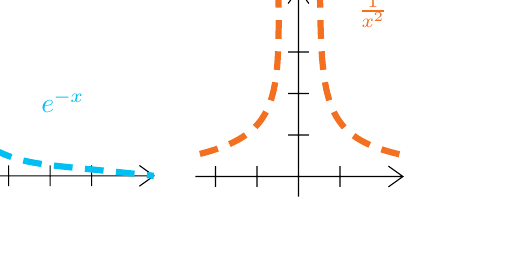
\begin{tikzpicture}[x=0.75pt,y=0.75pt,yscale=-1,xscale=1]
%uncomment if require: \path (0,577); %set diagram left start at 0, and has height of 577

% Plotting does not support converting to Tikz
% Plotting does not support converting to Tikz
%Shape: Axis 2D [id:dp9348304936758725] 
\draw  (50,390) -- (150,390)(60,300) -- (60,400) (143,385) -- (150,390) -- (143,395) (55,307) -- (60,300) -- (65,307) (80,385) -- (80,395)(100,385) -- (100,395)(120,385) -- (120,395)(55,370) -- (65,370)(55,350) -- (65,350)(55,330) -- (65,330) ;
\draw   ;
%Curve Lines [id:da14546745523662508] 
\draw [color={rgb, 255:red, 0; green, 192; blue, 243 }  ,draw opacity=1 ][line width=2.25]  [dash pattern={on 6.75pt off 4.5pt}]  (60,370) .. controls (87,386.33) and (86.33,383) .. (150,390) ;
%Shape: Axis 2D [id:dp9707581105998612] 
\draw  (170,390.33) -- (270,390.33)(219.67,300) -- (219.67,400) (263,385.33) -- (270,390.33) -- (263,395.33) (214.67,307) -- (219.67,300) -- (224.67,307) (239.67,385.33) -- (239.67,395.33)(199.67,385.33) -- (199.67,395.33)(179.67,385.33) -- (179.67,395.33)(214.67,370.33) -- (224.67,370.33)(214.67,350.33) -- (224.67,350.33)(214.67,330.33) -- (224.67,330.33) ;
\draw   ;
%Curve Lines [id:da6968754256630726] 
\draw [color={rgb, 255:red, 243; green, 112; blue, 33 }  ,draw opacity=1 ][line width=2.25]  [dash pattern={on 6.75pt off 4.5pt}]  (230,300) .. controls (230.67,354.67) and (231.67,371.67) .. (270,380) ;
%Curve Lines [id:da33814056645762214] 
\draw [color={rgb, 255:red, 243; green, 112; blue, 33 }  ,draw opacity=1 ][line width=2.25]  [dash pattern={on 6.75pt off 4.5pt}]  (210,300) .. controls (210.67,354.67) and (209.67,370.33) .. (170,380) ;

% Text Node
\draw (94.67,347.4) node [anchor=north west][inner sep=0.75pt]  [color={rgb, 255:red, 0; green, 192; blue, 243 }  ,opacity=1 ]  {$e^{-x}$};
% Text Node
\draw (247.33,301.4) node [anchor=north west][inner sep=0.75pt]  [color={rgb, 255:red, 243; green, 112; blue, 33 }  ,opacity=1 ]  {$\frac{1}{x^{2}}$};


\end{tikzpicture}
\end{center}
To address this integrals we will treat their troublesome points as \un{limits}.

\begin{Ex} 
To find the integral $I=\displaystyle\int_{-1}^{1}\frac{\dd x}{x^2}$, we must recognize that $\frac{1}{x^2}$ has a singularity at $x=0$. We must, separate the integral in two, and then take limits in both of them. We have 
\begin{align*}
  \int_{-1}^{1}\frac{\dd x}{x^2}&=\int_{-1}^{0}\frac{\dd x}{x^2}+\int_{0}^{1}\frac{\dd x}{x^2}
  &=\lim_{b\to 0^-}\int_{-1}^{b}\frac{\dd x}{x^2}+\lim_{a\to0^+}\int_{a}^{1}\frac{\dd x}{x^2}
\end{align*}
and the integrals inside the limits are our day-to-day, usual definite integrals. We evaluate them to see that 
$$I=\lim_{b\to0^-}\left(\frac{-1}{b}-\frac{-1}{(-1)}\right)+\lim_{a\to0^+}\left(\frac{-1}{1}-\frac{-1}{a}\right).$$
We can see that $b$'s limit is positive infinity and $a$'s limit is negative infinity. After solving the rest of the algebra we can see that the limit is infinite. 
\end{Ex}

\begin{Def}
We say that an improper integral \un{diverges} when its corresponding limit doesn't exist or is infinite.
\end{Def}

Let us take a look at the other example:

\begin{Ex}
  To calculate the integral $\displaystyle\int_0^{\infty}e^{-x}\dd x$, we first notice that the function $e^{-x}$ is continuous everywhere. So the only troublesome point is at infinity. We setup the integral as follows 
  \begin{align*}
    \int_0^{\infty}e^{-x}\dd x=\lim_{b\to\infty}\int_0^{b}e^{-x}\dd x&=\lim_{b\to\infty}(-e^{-b}-(-e^0))\\
    &=-\lim_{b\to\infty}e^{-b}+1=0+1=1.
  \end{align*}
  In this case we will say that $\displaystyle\int_0^{\infty}e^{-x}\dd x=1$ since the limit exists and its value is $1$.
\end{Ex}

\begin{Def}
  We say that an improper integral \un{converges} when its corresponding limit exists and it's finite. The value of that limit is the value we will assign to the improper integral.
  \end{Def}
  
  It may the case that we have both infinite limits! Consider the integral $\displaystyle\int_{-\infty}^\infty|x|e^{-x^2}\dd x$. While it would be tempting to consider that 
  $$\int_{-\infty}^\infty|x|e^{-x^2}\dd x=\lim_{a\to\infty}\int_{-a}^a|x|e^{-x^2}\dd x,$$
we can't do this. The behavior at each of the limits could be different.

  \begin{Ex}
    To evaluate the integral in question, we must separate by using any point in the middle which isn't a point of discontinuity.\par 
    The function $|x|e^{-x^2}\dd x$ is continuous everywhere so we pick $x=0$ as our point in the middle. Then
    $\int_{-\infty}^\infty|x|e^{-x^2}\dd x=\int_{-\infty}^0|x|e^{-x^2}\dd x+\int_{0}^\infty|x|e^{-x^2}\dd x$
    and now we take the limits.\par 
    But first, let's get rid of the absolute value by recalling that 
    $$|x|=\left\lbrace\begin{aligned}
      x,\ x>0\\
-x,\ x<0
    \end{aligned}\right.$$
    The integral in question becomes
    \begin{align*}
      &\lim_{r\to-\infty}\int_{r}^0(-x)e^{-x^2}\dd x+\lim_{s\to\infty}\int_{0}^sxe^{-x^2}\dd x\\
      =&\lim_{r\to-\infty}-\left(\frac{-1}{2}-\frac{-e^{-r^2}}{2}\right)+\lim_{s\to\infty}\left(\frac{-e^{-s^2}}{2}-\frac{-1}{2}\right)\\
      =&\frac{1}{2}-0+0+\frac{1}{2}=1.
    \end{align*}
    So in the end, we say that $\displaystyle\int_{-\infty}^\infty|x|e^{-x^2}\dd x=1$.
  \end{Ex}
  \begin{Rmk}
In cases like this one, if at least one of the integrals diverge, we will say that the whole integral diverges.
  \end{Rmk}
  \vfill\null
  \newpage
  \begin{ptcbP}
In groups, analyze the integral $\displaystyle\int_{1}^\infty\frac{\dd x}{x^2}$.
\vspace*{-0.5em}
\begin{enumerate}[i)]
  \itemsep=-0.4em 
  \item Sketch a graph of the function from $0$ to $\infty$.
  \item Evaluate the integral by taking the limit. Determine if it converges.
  \item Does the lower limit come into play? 
  \vspace*{-0.5em}
  \begin{itemize}
    \itemsep=-0.37em
    \item What happens if we switch $1$ for an $a$ and let $a>1$, for example $36$?
    \item Or if $a<1$? Maybe even $a<0$?
  \end{itemize}  
  \item How does the power of $x$ contribute? Consider switching the $2$ for a $p$. Examine different values of $p$: 
 \vspace*{-0.5em}
  \begin{itemize}
    \itemsep=-0.37em
    \item $p<2$, like $p=3/2$.
    \item Also $p=1$ or $p=1/2$.
    \item What happens with negative values of $p$? Like $p=-9$?
  \end{itemize}
 \end{enumerate}
  \end{ptcbP}

  \begin{ptcbP}
    Consider the integral $\displaystyle\int_{-3}^{4}\frac{\dd x}{x^3}$.\par 
    As in the last exercise analyze this integral's behavior.\vspace*{-0.5em}
    \begin{enumerate}[i)]
      \itemsep=-0.4em
      \item Change both limits to other values, including one where the interval doesn't contain zero. What happens in that case?
      \item What role does the exponent $3$ play? Change the values of the exponent and predict a general result.
    \end{enumerate}
  \end{ptcbP}


  \begin{ptcbP}
    Study the integral $\displaystyle\int_{0}^{a}\frac{\dd x}{\sqrt{a-x}}$, where $a\in\bR$.\vspace*{-0.5em}
    \begin{enumerate}[i)]
      \itemsep=-0.4em
      \item First consider a positive value of $a$, such as $a=2$. Does the integral 
      $$\int_{0}^{2}\frac{\dd x}{\sqrt{2-x}}$$
      converge or diverge? 
      \item Can you come up with a general result considering different values of $a$? This must \emph{all} numbers, not only the whole negative numbers.
    \end{enumerate}
  \end{ptcbP}

  \begin{ptcbP}
    Consider the function $f(t)=\frac{4t}{\sqrt[3]{t^2-4}}$.\vspace*{-0.5em}
    \begin{enumerate}[i)]
      \itemsep=-0.4em
      \item Find the points of discontinuity of $f$. Is this function discontinuous on a larger set?
      \item Determine if the integral 
      $$\int_1^2f(t)\dd t$$
      is improper or not. In case it is, determine if it converges or not. In the case it does, find its value.
    \end{enumerate}
  \end{ptcbP}

  \begin{ptcbP}
    Consider the function $f(z)=\frac{1}{z^2}e^{\frac{1}{z}}$.
    \vspace*{-0.5em}
    \begin{enumerate}[i)]
      \itemsep=-0.4em
      \item Where is this function discontinuous?
      \item If possible, find the value of the integral 
      $$\int_{-\infty}^0f(z)\dd z.$$
    \end{enumerate}
  \end{ptcbP}

  \begin{ptcbP}
    How does the integral $\displaystyle\int_{-\infty}^{1}{\sqrt{a-y}}\ \dd y$, where $a\in\bR$.\vspace*{-0.5em}
    \begin{enumerate}[i)]
      \itemsep=-0.4em
      \item Suppose $a$ is positive, such as $a=9$. Is the function continuous over the specified domain of integration? What if we switched the $1$ to a $10$?
      \item If we replace the $1$ for a real number $b$, what can you say about the convergence of the integral? \emph{The answer must depend on $a$ and $b$}. 
    \end{enumerate}
  \end{ptcbP}

\end{multicols}
\end{document} 